
This stone is based on Burstedde et al (2008) \cite{bugg08}:

\begin{center}
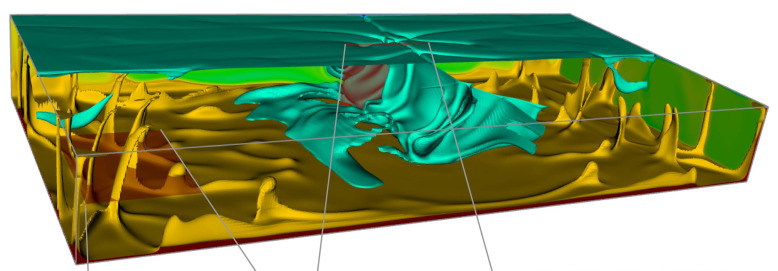
\includegraphics[width=12cm]{python_codes/fieldstone_88/images/bugg08}\\
{\captionfont Taken from \cite{bugg08}.}
\end{center}

This stone solves the dimensionless thermo-mechanical equations:
\begin{eqnarray}
\vec\nabla\cdot\vec\upnu &=& 0 \\
-\vec\nabla p + \vec\nabla \cdot [ 2 \eta(T,\dot{\varepsilon}_e,y) \dot{\bm \varepsilon} ] &=& Ra\; T \vec{e}_y \\
\frac{\partial T}{\partial t} + \vec\upnu \cdot \vec\nabla T &=& \Delta T
\end{eqnarray}
with $\dot{\varepsilon}_e$ is the effective strain rate and the viscosity is given by 
\[
\eta(T,\dot{\varepsilon}_e,y) =
\left\{
\begin{array}{c}
\min \left(  \frac{\sigma_y}{2 \dot{\varepsilon}_e} , 10\exp(-6.9T)  \right) \qquad y\le 0.9 \\
0.8 \exp(-6.9T) \qquad\quad  0.77\le y \le 0.9 \\
50 \exp(-6.9T) \qquad\quad y \le 0.77 
\end{array}
\right.
\]

\begin{center}
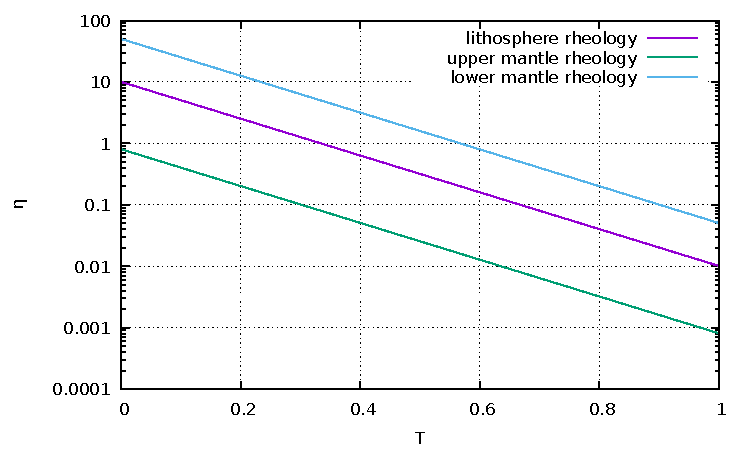
\includegraphics[width=8cm]{python_codes/fieldstone_88/images/visc.pdf}\\
{\captionfont Dimensionless viscosity values as a function of the dimensionless temperature.}
\end{center}

In the paper the value of $\sigma_y$ is not specified, nor is the Rayleigh number (although 
they mention it is between $10^6$ and $10^9$).
Their box is 8x4x1 and temperatures range from 0 at the top to 1 at the bottom.
In this case 3D modeling is out of the question here so we restrict ourselves to 2D with a 4x1 domain. 




To start with, w implement the advection-diffusion equation without stabilisation. The initial temperature
boundary conditions are such that a large upwelling is created


We then apply the Lenardic \& Kaula (1993) \cite{leka93} filter, as explained in Section~\ref{sec:compfield}.
\begin{enumerate}
\item Compute the initial sum $S_0$ of all values of $C$.
\item Find the minimal value $C_{min}$ below 0.
\item Find the maximal value $C_{max}$ above 1.
\item Set $C_i=0$ if $C_i \leq |C_{min}|$.
\item Set $C_i=1$ if $C_i \geq 2-C_{max}$. 
\item Compute the sum $S_1$ of all values of $C$
\item Compute the number $num$ of $0 < C_i < 1$.
\item Add $(S_1-S_0)/num$ to all $0<C_i<1$
\end{enumerate}


The filter is designed to prevent under- and overshoot but it cannot remove the oscillations between 0 and 1.
It therefore cannot 'cure' alone the poor quality of the solution within these bounds.
\begin{center}
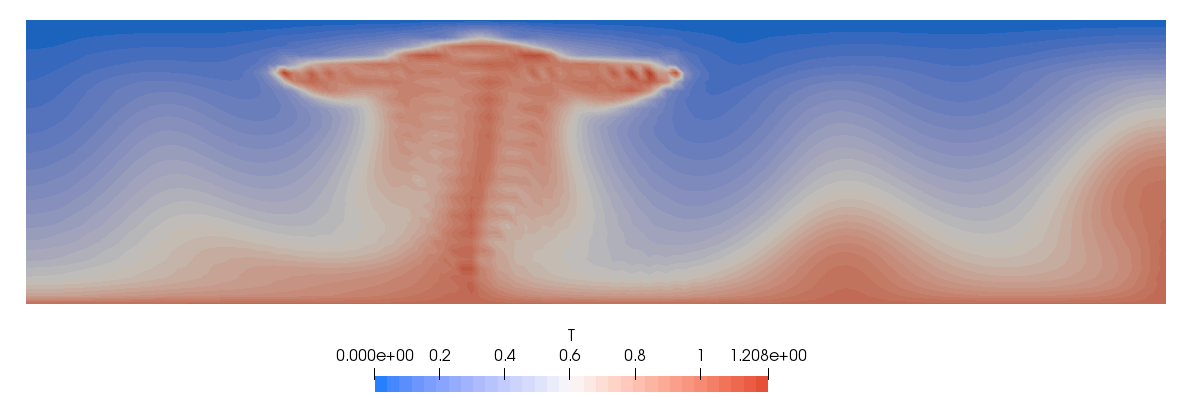
\includegraphics[width=9cm]{python_codes/fieldstone_88/results/without}\\
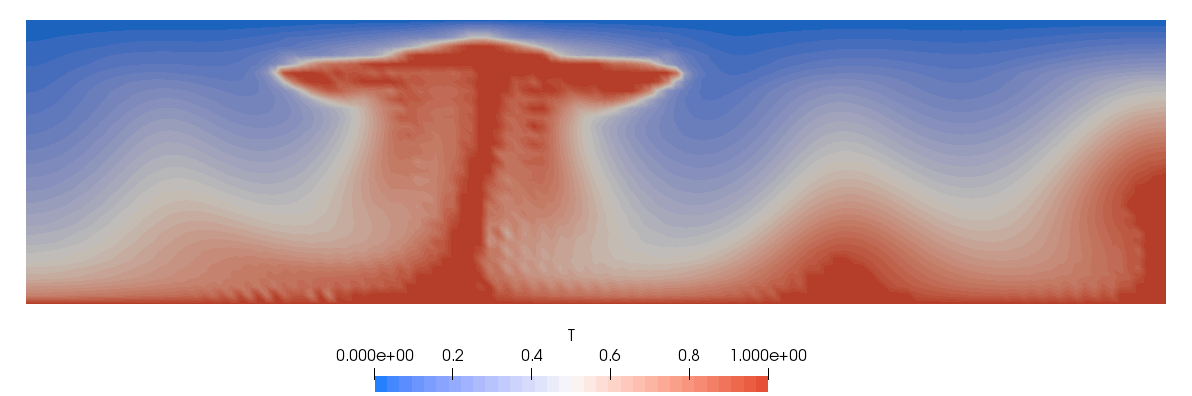
\includegraphics[width=9cm]{python_codes/fieldstone_88/results/with}\\
{\captionfont Top: no filter, bottom: with filter. 64x16, CFL=0.5\\ Notice the different scales.}
\end{center}


We leave the filter on and now focus on the importance of resolution. All other things equal we increase
resolution from 64x16 to 128x32 and run all models up to (dimensionless) time 0.00015 with $Ra=10^6$.




 



\vspace{3cm}

Q: If I want to start from adiabatic temp gradient, how to compute it, how to make it dimensionless?

pressure nullspace
